\documentclass[slidetop, 10pt]{beamer}\usepackage{graphicx, color}
%% maxwidth is the original width if it is less than linewidth
%% otherwise use linewidth (to make sure the graphics do not exceed the margin)
\makeatletter
\def\maxwidth{ %
  \ifdim\Gin@nat@width>\linewidth
    \linewidth
  \else
    \Gin@nat@width
  \fi
}
\makeatother

\IfFileExists{upquote.sty}{\usepackage{upquote}}{}
\definecolor{fgcolor}{rgb}{0.2, 0.2, 0.2}
\newcommand{\hlnumber}[1]{\textcolor[rgb]{0,0,0}{#1}}%
\newcommand{\hlfunctioncall}[1]{\textcolor[rgb]{0.501960784313725,0,0.329411764705882}{\textbf{#1}}}%
\newcommand{\hlstring}[1]{\textcolor[rgb]{0.6,0.6,1}{#1}}%
\newcommand{\hlkeyword}[1]{\textcolor[rgb]{0,0,0}{\textbf{#1}}}%
\newcommand{\hlargument}[1]{\textcolor[rgb]{0.690196078431373,0.250980392156863,0.0196078431372549}{#1}}%
\newcommand{\hlcomment}[1]{\textcolor[rgb]{0.180392156862745,0.6,0.341176470588235}{#1}}%
\newcommand{\hlroxygencomment}[1]{\textcolor[rgb]{0.43921568627451,0.47843137254902,0.701960784313725}{#1}}%
\newcommand{\hlformalargs}[1]{\textcolor[rgb]{0.690196078431373,0.250980392156863,0.0196078431372549}{#1}}%
\newcommand{\hleqformalargs}[1]{\textcolor[rgb]{0.690196078431373,0.250980392156863,0.0196078431372549}{#1}}%
\newcommand{\hlassignement}[1]{\textcolor[rgb]{0,0,0}{\textbf{#1}}}%
\newcommand{\hlpackage}[1]{\textcolor[rgb]{0.588235294117647,0.709803921568627,0.145098039215686}{#1}}%
\newcommand{\hlslot}[1]{\textit{#1}}%
\newcommand{\hlsymbol}[1]{\textcolor[rgb]{0,0,0}{#1}}%
\newcommand{\hlprompt}[1]{\textcolor[rgb]{0.2,0.2,0.2}{#1}}%

\usepackage{framed}
\makeatletter
\newenvironment{kframe}{%
 \def\at@end@of@kframe{}%
 \ifinner\ifhmode%
  \def\at@end@of@kframe{\end{minipage}}%
  \begin{minipage}{\columnwidth}%
 \fi\fi%
 \def\FrameCommand##1{\hskip\@totalleftmargin \hskip-\fboxsep
 \colorbox{shadecolor}{##1}\hskip-\fboxsep
     % There is no \\@totalrightmargin, so:
     \hskip-\linewidth \hskip-\@totalleftmargin \hskip\columnwidth}%
 \MakeFramed {\advance\hsize-\width
   \@totalleftmargin\z@ \linewidth\hsize
   \@setminipage}}%
 {\par\unskip\endMakeFramed%
 \at@end@of@kframe}
\makeatother

\definecolor{shadecolor}{rgb}{.97, .97, .97}
\definecolor{messagecolor}{rgb}{0, 0, 0}
\definecolor{warningcolor}{rgb}{1, 0, 1}
\definecolor{errorcolor}{rgb}{1, 0, 0}
\newenvironment{knitrout}{}{} % an empty environment to be redefined in TeX

\usepackage{alltt}
\usepackage[T1]{fontenc}
\usepackage[utf8]{inputenc}
\usepackage{default}
\usepackage{array}
\usepackage{multirow}
\usepackage{lmodern}
\usepackage[frenchb]{babel}
\usetheme{Antibes}

\usecolortheme{beaver}
\title{Éléments de cartographie sous R}
\subtitle{RUG INSEE}
\author{Joël Gombin}
\institute{CURAPP - UPJV}
\date{11 octobre 2012}
\usepackage{graphicx}
\usepackage[fixlanguage]{babelbib}
\selectbiblanguage{french}
\setbeamertemplate{navigation symbols}{}
\usepackage{listings}

\usepackage{color}
\usepackage{alltt}
\usepackage{hyperref}

\ifdefined\knitrout
  \renewenvironment{knitrout}{\begin{tiny}}{\end{tiny}}
\else
\fi

\definecolor{links}{HTML}{2A1B81}
\hypersetup{colorlinks,linkcolor=,urlcolor=links}



\AtBeginSection[] 
{ 
  \begin{frame}[plain]{Plan} 
    \tableofcontents[currentsection, hideothersubsections] 
  \end{frame} 
} 



\begin{document}

\frame{\titlepage}

\section{Quelques éléments sur la cartographie}

\begin{frame}
\frametitle{Introduction : notions de base de cartographie}



\begin{block}{Carte raster}
Carte composée de pixels : par exemple une photo satellite. L'information est représentée par la couleur du pixel, lui-même porteur d'une information géographique (coordonnées \verb!x! et \verb!y!).
\end{block}

\begin{block}{Carte vectorielle}
Carte composée d'éléments : points, lignes, courbes, polygones... Ces éléments constituent en eux-même une information géographique (ils ont des coordonnées), à laquelle on peut  ajouter une information supplémentaire (par exemple en coloriant un polygone).
\end{block}

\end{frame}

\begin{frame}
\frametitle{Notions de base de cartographie}

Si on s'en tient aux cartes vectorielles, seules traitées ici, pour faire une carte il faut :

\begin{itemize}
\item un fond de carte (dans un format vectoriel : une simple image ne suffit pas) (généralement associé à une projection, permettant le passage d'une sphère à un plan. E.g. : \href{http://geekisawesome.com/1865/what-map-projections-say-about-you/}{Mercator}).
\item des données se rapportant aux objets de cette carte
\item un identifiant commun à ces deux ensembles.
\end{itemize}

\end{frame}


\section{La cartographie dans R}

\begin{frame}
\frametitle{La cartographie dans R}

Dans R, les cartes sont des objets dotés d'une structure complexe. Il existe plusieurs approches, mais la plus répandue consiste à utiliser la classe d'objets \verb!SpatialPolygonsDataFrame!. C'est le package \verb!sp! qui définit cette classe, qui contient aussi bien des données géographiques (coordonnées des éléments) que des données sur ces objets.

Une bonne pratique consiste à séparer les donnnées portant sur les éléments (coordonnées mais aussi identifiants, par exemple) et celles qu'on souhaite cartographier dans deux objets distincts.

Par ailleurs, le package \verb!ggplot2! propose également une fonction pour représenter des cartes raster ou choroplèthes (\verb!geom\_map()!), mais est lent et peu souple pour cette tâche. Il semble toutefois que le choix de la projection soit plus aisé.

\end{frame}

\begin{frame}
\frametitle{Les outils du package \verb!rgrs!}
Dans le cadre de cette introduction, je vais présenter essentiellement les outils du package \verb!rgrs! développé par \href{http://alea.fr.eu.org/}{Julien Barnier}. Ils sont à la fois faciles à utiliser et relativement puissants. Une fois la logique assimilée, il sera aisé d'aller plus loin si nécessaire.

\begin{knitrout}\tiny
\definecolor{shadecolor}{rgb}{0.969, 0.969, 0.969}\color{fgcolor}\begin{kframe}
\begin{alltt}
\hlfunctioncall{library}(rgrs)
\hlfunctioncall{library}(sp)
\hlfunctioncall{library}(maptools)
\end{alltt}
\end{kframe}
\end{knitrout}


\end{frame}

\section{Importer des données géographiques}
\begin{frame}[fragile]
\frametitle{Importer des données géographiques}

Il existe de nombreux formats de données cartographiques, mais le plus répandu est le \verb!shapefile!. Une carte est contenue dans un ensemble de fichiers portant tous le même nom mais dotés d'extensions différentes (\verb!.shp!, \verb!.dbf!, \verb!.prj!...). 

\begin{knitrout}\tiny
\definecolor{shadecolor}{rgb}{0.969, 0.969, 0.969}\color{fgcolor}\begin{kframe}
\begin{alltt}
\hlfunctioncall{library}(rgdal)
picardie <- \hlfunctioncall{readOGR}(\hlstring{"donnees/"}, \hlstring{"picardie"})
\end{alltt}
\begin{verbatim}
## OGR data source with driver: ESRI Shapefile 
## Source: "donnees/", layer: "picardie"
## with 2291 features and 18 fields
## Feature type: wkbPolygon with 2 dimensions
\end{verbatim}
\begin{alltt}
picardie\$STATUT <- \hlfunctioncall{as.factor}(\hlfunctioncall{iconv}(picardie\$STATUT, from = \hlstring{"latin1"}, to = \hlstring{"utf8"}))  ## traitement de problèmes d'encodage
picardie\$codeINSEE <- \hlfunctioncall{as.character}(picardie\$INSEE_COM)
\end{alltt}
\end{kframe}
\end{knitrout}

\end{frame}


\section{Manipuler des objets spatiaux}
\begin{frame}[fragile]
\frametitle{Avoir des informations sur une carte et la représenter}
\begin{knitrout}\tiny
\definecolor{shadecolor}{rgb}{0.969, 0.969, 0.969}\color{fgcolor}\begin{kframe}
\begin{alltt}
\hlfunctioncall{summary}(picardie)
\end{alltt}
\end{kframe}
\end{knitrout}

\begin{knitrout}\tiny
\definecolor{shadecolor}{rgb}{0.969, 0.969, 0.969}\color{fgcolor}\begin{kframe}
\begin{alltt}
\hlfunctioncall{require}(sp)
\hlfunctioncall{plot}(picardie)
\end{alltt}
\end{kframe}
\end{knitrout}


\begin{knitrout}\tiny
\definecolor{shadecolor}{rgb}{1, 1, 1}\color{fgcolor}

{\centering 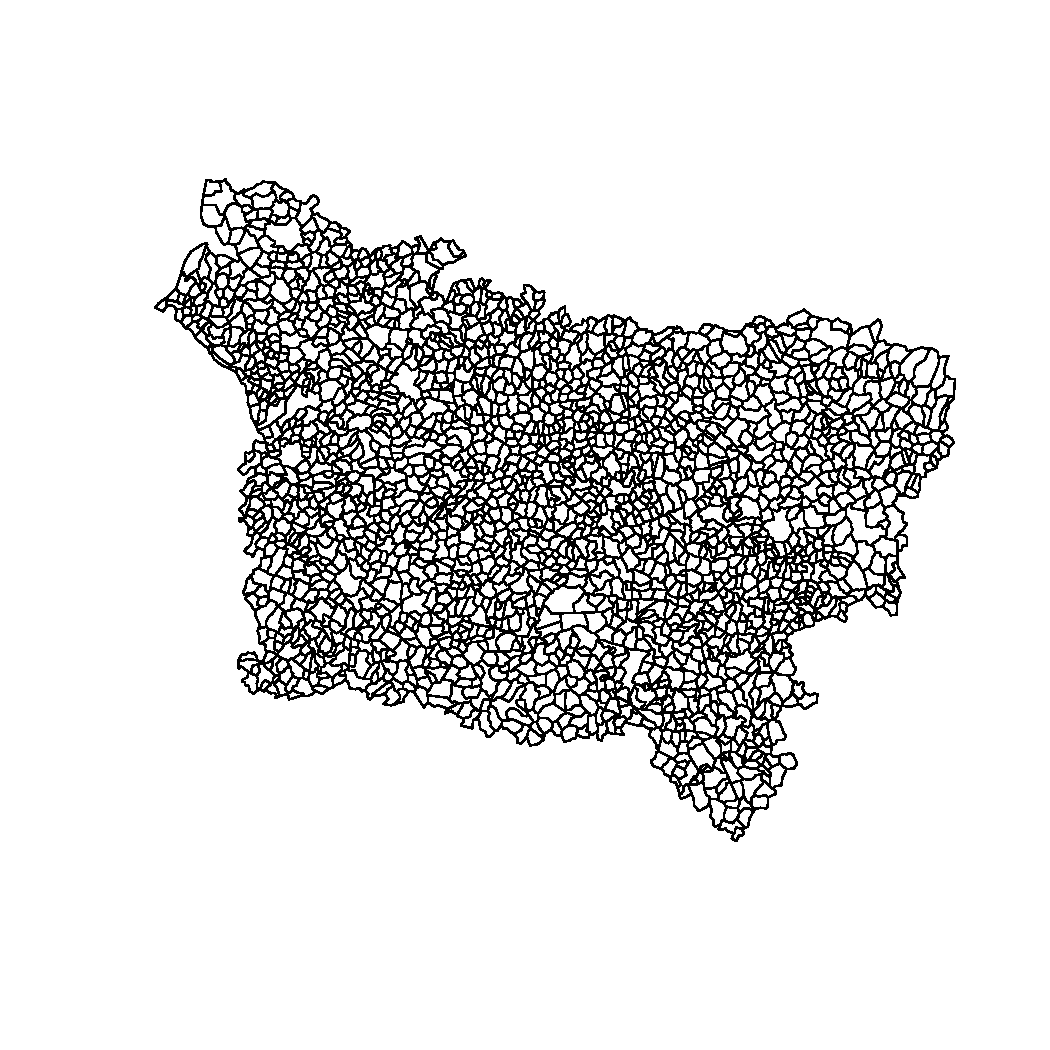
\includegraphics[width=.7\linewidth]{images/shp4} 

}


\end{knitrout}


\end{frame}

\begin{frame}[fragile]
\frametitle{Manipuler une carte}

Une carte est donc un objet de type \verb!SpatialPolygonsDataFrame!. Il contient plusieurs ensemble de données ; généralement, le seul qu'on manipule directement est le slot \verb!@data!, qui contient les données sur les objets géographiques. 

\begin{knitrout}\tiny
\definecolor{shadecolor}{rgb}{0.969, 0.969, 0.969}\color{fgcolor}\begin{kframe}
\begin{alltt}
\hlfunctioncall{names}(picardie@data)
\end{alltt}
\begin{verbatim}
##  [1] "ID_GEOFLA"  "CODE_COMM"  "INSEE_COM"  "NOM_COMM"   "STATUT"    
##  [6] "X_CHF_LIEU" "Y_CHF_LIEU" "X_CENTROID" "Y_CENTROID" "Z_MOYEN"   
## [11] "SUPERFICIE" "POPULATION" "CODE_CANT"  "CODE_ARR"   "CODE_DEPT" 
## [16] "NOM_DEPT"   "CODE_REG"   "NOM_REGION" "codeINSEE"
\end{verbatim}
\begin{alltt}
\hlfunctioncall{summary}(picardie@data\$NOM_DEPT)
\end{alltt}
\begin{verbatim}
## AISNE  OISE SOMME 
##   816   693   782
\end{verbatim}
\end{kframe}
\end{knitrout}

\end{frame}

\begin{frame}[fragile]
\frametitle{Manipuler une carte}
De plus, on manipule une carte comme n'importe quel dataframe :

\begin{knitrout}\tiny
\definecolor{shadecolor}{rgb}{0.969, 0.969, 0.969}\color{fgcolor}\begin{kframe}
\begin{alltt}
somme <- picardie[picardie@data\$CODE_DEPT == \hlstring{"80"}, ]
\end{alltt}
\end{kframe}
\end{knitrout}


Le package \verb!sp! offre de plus des outils pour facilement manipuler plusieurs couches cartographiques (par exemple étudier l'intersection de plusieurs ensembles d'éléments géographiques).

Enfin, on sauve et charge cet objet comme n'importe quel autre :

\begin{knitrout}\tiny
\definecolor{shadecolor}{rgb}{0.969, 0.969, 0.969}\color{fgcolor}\begin{kframe}
\begin{alltt}
\hlfunctioncall{save}(picardie, file = \hlstring{"donnees/picardie.Rdata"})
\hlfunctioncall{load}(\hlstring{"picardie.Rdata"})
\end{alltt}
\end{kframe}
\end{knitrout}


\end{frame}
\begin{frame}[fragile]
\frametitle{Agréger des éléments cartographiques}
On a parfois besoin de regrouper entre eux des polygones. Par exemple, de ma carte communale, je veux tirer une carte des départements. 

\begin{knitrout}\tiny
\definecolor{shadecolor}{rgb}{0.969, 0.969, 0.969}\color{fgcolor}\begin{kframe}
\begin{alltt}
\hlfunctioncall{require}(gpclib)
\hlfunctioncall{gpclibPermit}()
\end{alltt}
\begin{verbatim}
## [1] TRUE
\end{verbatim}
\begin{alltt}
\hlfunctioncall{require}(maptools)
dpts <- \hlfunctioncall{unionSpatialPolygons}(picardie, IDs = picardie@data\$CODE_DEPT)
\hlfunctioncall{plot}(dpts)
\end{alltt}
\end{kframe}

{\centering 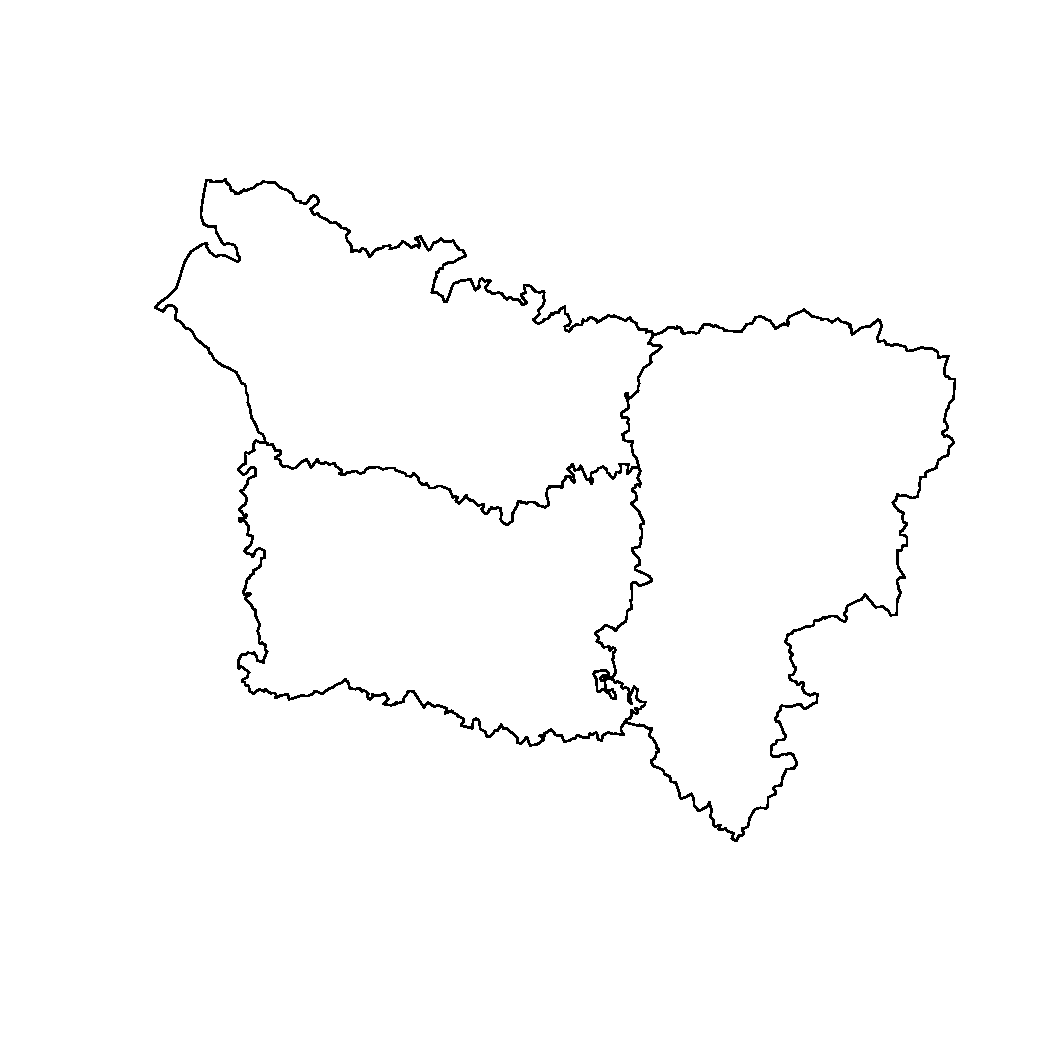
\includegraphics[width=.4\linewidth]{images/union} 

}


\end{knitrout}

\end{frame}

\section{Cartes choroplèthes}
\begin{frame}[fragile]
\frametitle{Représenter des proportions : les cartes choroplèthes}

L'intérêt d'une carte n'est généralement pas de simplement représenter des objets géographiques mais d'y associer de l'information. Il y a de multiples manières de le faire ; on se concentrera ici sur les cartes choroplèthes, dans lesquelles les polygones sont coloriées en fonction de la variable d'intérêt.

On commence par vérifier qu'on a bien un identidiant commun à nos données et à notre carte :

\begin{knitrout}\tiny
\definecolor{shadecolor}{rgb}{0.969, 0.969, 0.969}\color{fgcolor}\begin{kframe}
\begin{alltt}
\hlfunctioncall{load}(\hlstring{"donnees/mini_picardie.Rdata"})
\hlfunctioncall{head}(mini_picardie\$CODE_COMMU)
\end{alltt}
\begin{verbatim}
## [1] 001 002 003 004 005 006
## 908 Levels:     001 002 003 004 005 006 007 008 009 010 011 012 013 ... 909
\end{verbatim}
\begin{alltt}
\hlcomment{# Non, donc on recode :}
mini_picardie\$codeINSEE <- \hlfunctioncall{paste}(\hlfunctioncall{as.character}(mini_picardie\$CODE_D_PAR), \hlfunctioncall{as.character}(mini_picardie\$CODE_COMMU), 
    sep = \hlstring{""})
\end{alltt}
\end{kframe}
\end{knitrout}


\end{frame}

\begin{frame}
\frametitle{Représenter des proportions : les cartes choroplèthes}
Par facilité, on ne va travailler que sur la Somme. On utilise la fonction \verb!carte.prop! du package \verb!rgrs! :

\begin{knitrout}\tiny
\definecolor{shadecolor}{rgb}{0.969, 0.969, 0.969}\color{fgcolor}\begin{kframe}
\begin{alltt}
somme <- picardie[picardie@data\$CODE_DEPT == \hlstring{"80"}, ]
\hlfunctioncall{carte.prop}(somme, mini_picardie, varname = \hlstring{"AbsIns"}, sp.key = \hlstring{"codeINSEE"}, data.key = \hlstring{"codeINSEE"}, 
    at = \hlfunctioncall{quantile}(mini_picardie\$AbsIns, \hlfunctioncall{c}(0, 0.25, 0.5, 0.75, 1)))
\end{alltt}
\end{kframe}

{\centering 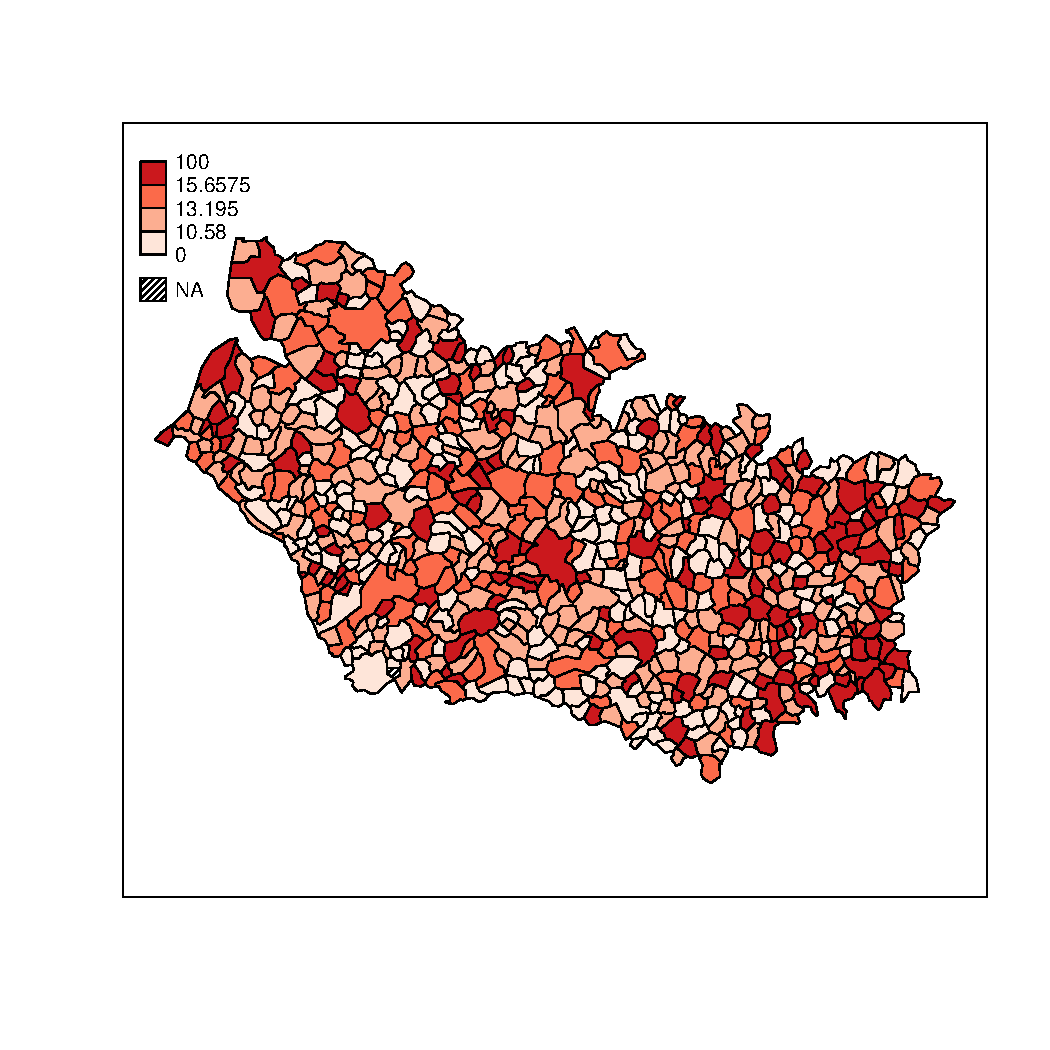
\includegraphics[width=.55\linewidth]{images/carteprop} 

}


\end{knitrout}



\end{frame}

\begin{frame}[fragile]
\frametitle{Paramétrer une carte choroplèthe}

La fonction \verb!carte.prop! prend une série d'arguments, que vous pouvez tester.

Par ailleurs, pour le choix des couleurs, on peut s'aider du site \url{http://www.colorbrewer2.org}. Les arguments \verb!palette.pos! et \verb!palette.neg! de \verb!carte.prop! prennent les noms proposés sur le site. 
\end{frame}

\section{Représenter des effectifs}
\begin{frame}
\frametitle{Représenter des effectifs}

Admettons que nous voulions représenter les effectifs des communes de la Somme. 


\begin{knitrout}\tiny
\definecolor{shadecolor}{rgb}{0.969, 0.969, 0.969}\color{fgcolor}\begin{kframe}
\begin{alltt}
\hlfunctioncall{carte.eff}(somme, mini_picardie, varname = \hlstring{"Population"}, sp.key = \hlstring{"codeINSEE"}, 
    data.key = \hlstring{"codeINSEE"})
\end{alltt}
\end{kframe}

{\centering 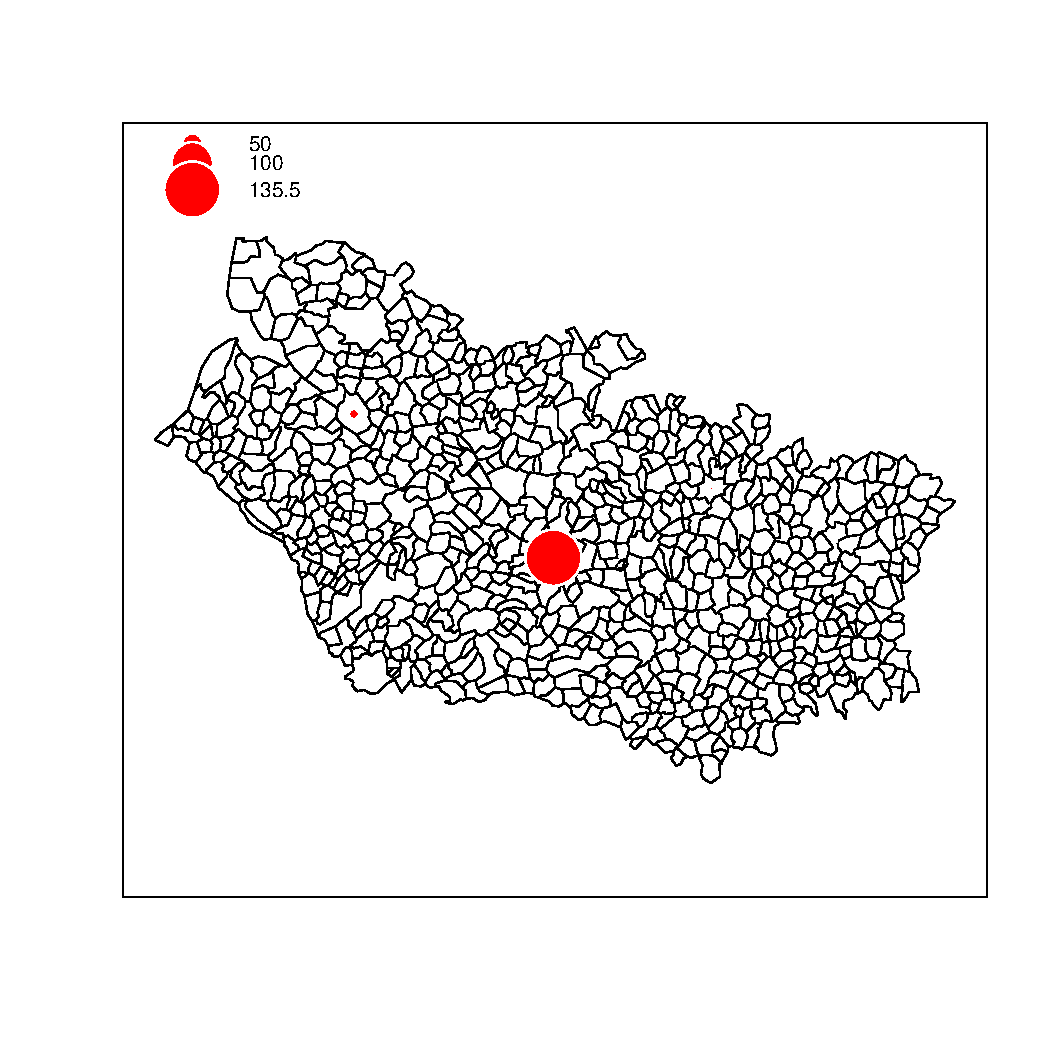
\includegraphics[width=.55\linewidth]{images/carteeff} 

}


\end{knitrout}


\end{frame}
\section{Représenter une variable catégorielle}
\begin{frame}[fragile]
\frametitle{Représenter une variable catégorielle}
La syntaxe est toujours très proche, on utilise cette fois-ci la fonction \verb!carte.qual! :

\begin{knitrout}\tiny
\definecolor{shadecolor}{rgb}{0.969, 0.969, 0.969}\color{fgcolor}\begin{kframe}
\begin{alltt}

pal <- \hlfunctioncall{c}(\hlstring{"orange"}, \hlstring{"yellow"}, \hlstring{"light green"}, \hlstring{"red"})
\hlfunctioncall{carte.qual}(somme, mini_picardie, varname = \hlstring{"type_urbain"}, sp.key = \hlstring{"codeINSEE"}, 
    data.key = \hlstring{"codeINSEE"}, palette = pal, posleg = \hlstring{"bottomleft"}, main = \hlstring{"Le découpage en ZAUER en Picardie"}, 
    sub = \hlstring{"source : INSEE."})
\end{alltt}
\end{kframe}

{\centering 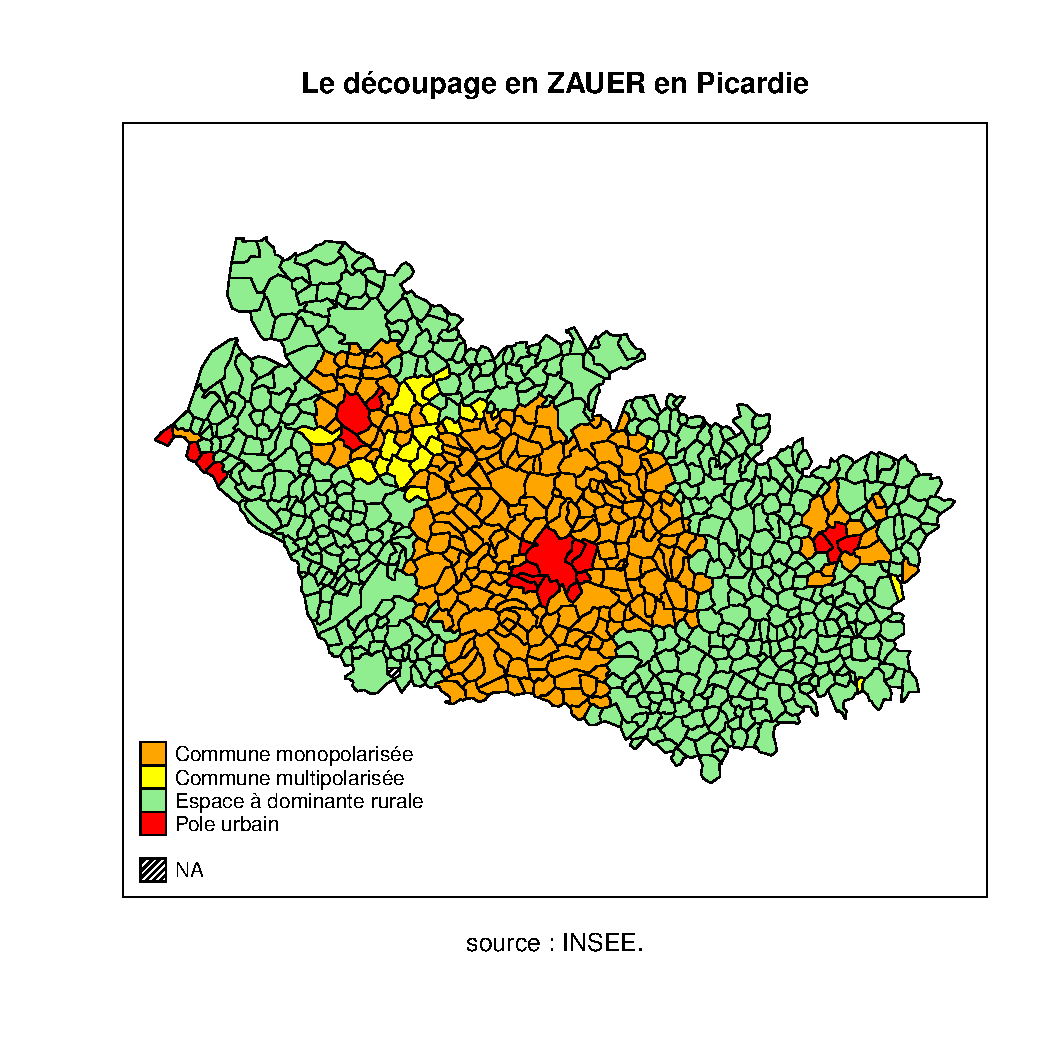
\includegraphics[width=.5\linewidth]{images/cartequal} 

}


\end{knitrout}


\end{frame}

\section{Quelques subtilités supplémentaires...}
\begin{frame}[fragile]
\frametitle{Rajouter des bordures}
Imaginons que nous voulions rajouter les découpages des arrondissements. Il nous faut d'abord créer des éléments correspondants, et ensuite les ajouter.

\begin{knitrout}\tiny
\definecolor{shadecolor}{rgb}{0.969, 0.969, 0.969}\color{fgcolor}\begin{kframe}
\begin{alltt}
arrdts <- \hlfunctioncall{unionSpatialPolygons}(somme, IDs = somme@data\$CODE_ARR)
\hlfunctioncall{carte.qual}(somme, mini_picardie, varname = \hlstring{"type_urbain"}, sp.key = \hlstring{"codeINSEE"}, 
    data.key = \hlstring{"codeINSEE"}, palette = pal, posleg = \hlstring{"bottomleft"}, main = \hlstring{"Le découpage en ZAUER en Picardie"}, 
    sub = \hlstring{"source : INSEE."})
\hlfunctioncall{plot}(arrdts, lwd = 5, border = \hlstring{"red"}, add = TRUE)
\end{alltt}
\end{kframe}

{\centering 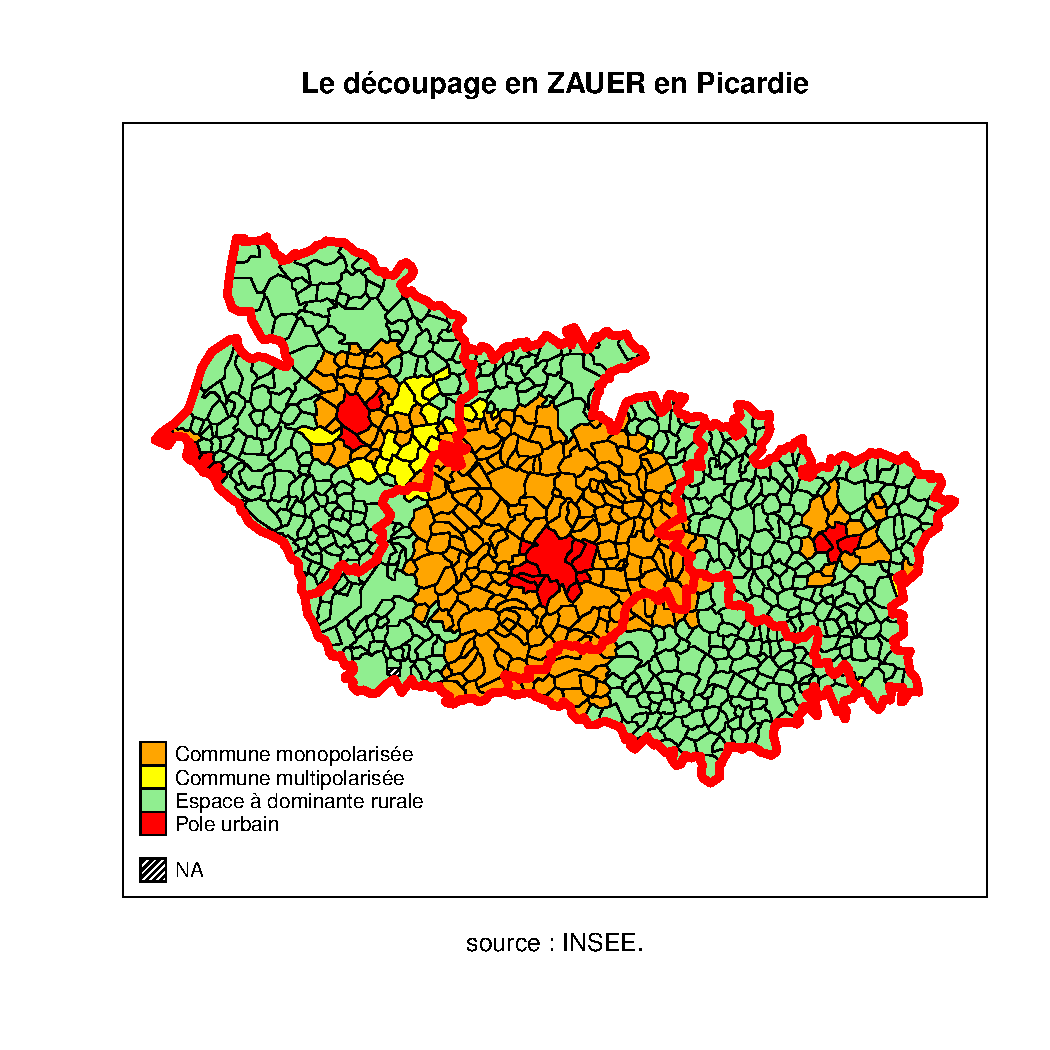
\includegraphics[width=.45\textwidth]{images/fusion} 

}


\end{knitrout}



\end{frame}

\begin{frame}[fragile]
\frametitle{Faire une carte en coloration continue}

Le "truc" consiste à passer autant de breaks, et de couleurs, à la fonction que de valeurs différentes de la variable continue représentée. Pour cela on choisit les couleurs qu'on veut pour sa palette (palette séquentielle ou divergente), puis on crée une palette de \verb!n! valeurs à partir d'un certain nombre de points. On passe \verb!pal(n)! en argument de \verb!carte.prop!.

\begin{knitrout}\tiny
\definecolor{shadecolor}{rgb}{0.969, 0.969, 0.969}\color{fgcolor}\begin{kframe}
\begin{alltt}
\hlfunctioncall{library}(RColorBrewer)
colors <- \hlfunctioncall{brewer.pal}(6, \hlstring{"RdBu"})
pal <- \hlfunctioncall{colorRampPalette}(colors)
\hlfunctioncall{carte.prop}(picardie, mini_picardie, \hlstring{"revenu.fiscal.moyen"}, sp.key = \hlstring{"codeINSEE"}, 
    data.key = \hlstring{"codeINSEE"}, at = \hlfunctioncall{as.integer}(\hlfunctioncall{levels}(\hlfunctioncall{as.factor}(mini_picardie\$revenu.fiscal.moyen))), 
    border = \hlstring{"transparent"}, palette = \hlfunctioncall{pal}(\hlfunctioncall{length}(\hlfunctioncall{levels}(\hlfunctioncall{as.factor}(mini_picardie\$revenu.fiscal.moyen)))), 
    posleg = \hlstring{"none"}, main = \hlstring{"Le revenu fiscal moyen des ménages par communes"})
\hlfunctioncall{plot}(dpts, add = T)
\end{alltt}
\end{kframe}
\end{knitrout}

\end{frame}

\begin{frame}
\frametitle{Faire une carte en coloration continue}
\begin{knitrout}\tiny
\definecolor{shadecolor}{rgb}{0.969, 0.969, 0.969}\color{fgcolor}

{\centering 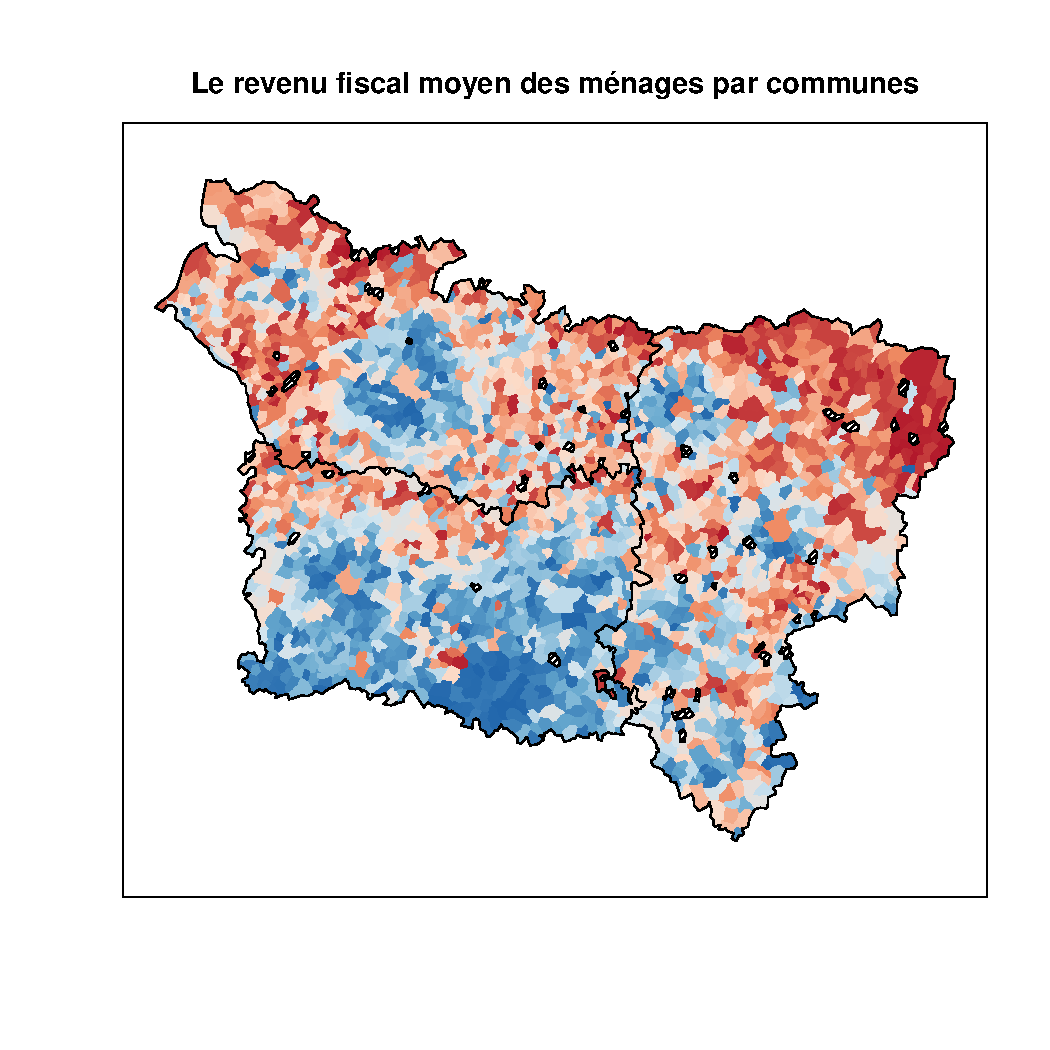
\includegraphics[width=.8\textwidth]{images/coloration} 

}


\end{knitrout}


\end{frame}
\section*{Conclusion}
\begin{frame}
\frametitle{Conclusion}

La cartographie dans R est assez simple, en tout cas pour des tâches simples, et surtout offre à la fois beaucoup de souplesse tout en utilisant une syntaxe commune avec la manipulation de données. 

De plus, en scriptant, on peut produire très rapidement de très nombreuses cartes, soit de différents territoires, soit de différentes variables.


Pour la route, le blog d'un géographe anglais produisant de magnifiques cartes sous R : \url{http://spatialanalysis.co.uk/}.


Présentation disponible sur : \url{https://github.com/joelgombin/SeminR}

\end{frame}

\end{document}
